\documentclass[a1paper,portrait,margin=20mm]{tikzposter}
\input{socceranalytics} % configure for poster session


% identify your project and choose a main color
% =================================================================
\project{K4}{VIL}{AD}
\students{%
  Philip Beck,
  Philip Olson,
  Giovanni Di Nunzio,
  Lukas Schenker
 } 
\maincolor{green}
% =================================================================
% ETH palette: blue,green,red,bronze,purple,petrol,black,grey
% or define one of your own with \definecolor{mycolor}{HTML}{ffff00}


% =================================================================
\begin{document}\maketitle 
% =================================================================

  % -- a wide block
  \block{Villarreal Report Summar for Attack \& Defense}
   {
	   Villarreal CF faced a highly challenging 2025/26 UEFA Champions League campaign, struggling with defensive vulnerabilities during transition moments. This project analyzes their tactical framework, specifically examining how their in-possession organization directly impacted their overall defensive stability. By combining event and tracking data, we map their build-up patterns to identify structural flaws and pinpoint primary turnover zones. Ultimately, this research provides actionable insights to help optimize their spatial dominance and mitigate the dangers of possession losses.
   }

  % -- two columns of blocks
  \begin{columns} 
  \column{0.49}
  \block{Pitch Control}
	  {
		  Villarreal exhibits a patient, possession-based style characterized by heavy goalkeeper involvement and concentrated ball circulation in the central midfield. Our spatial analysis reveals a distinct lack of control deep in the opponent's half, highlighting a heavy reliance on short, horizontal ground passes to manage the tempo of the game. However, this deep-seated possession often leaves the team struggling to penetrate the final third efficiently. Occasional long passes from the backline are utilized merely as situational tools to bypass high pressure rather than as a primary attacking mechanism.
	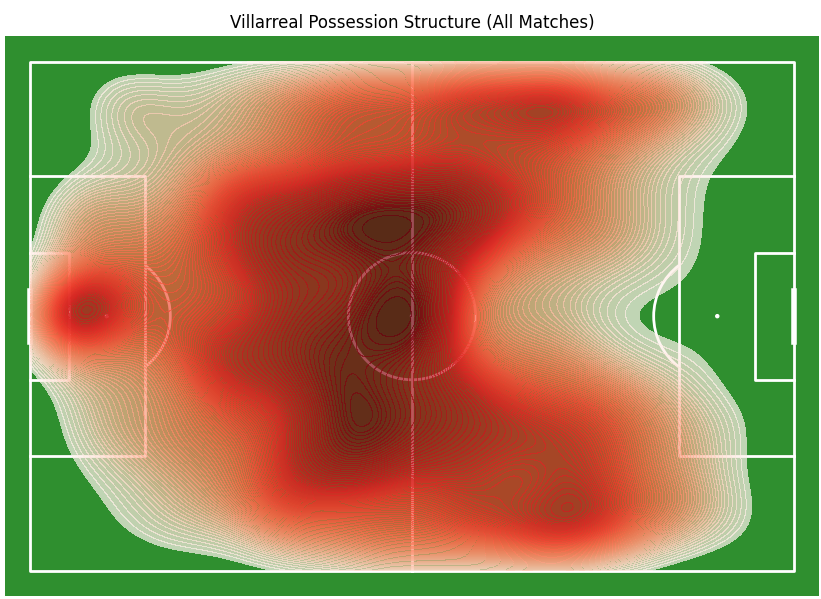
\includegraphics[width=50ex]{pitch_control}\hfill
	}

  % right column is wider
  \column{0.51}
    \block{Turnover Types and their Dangers}
     {
      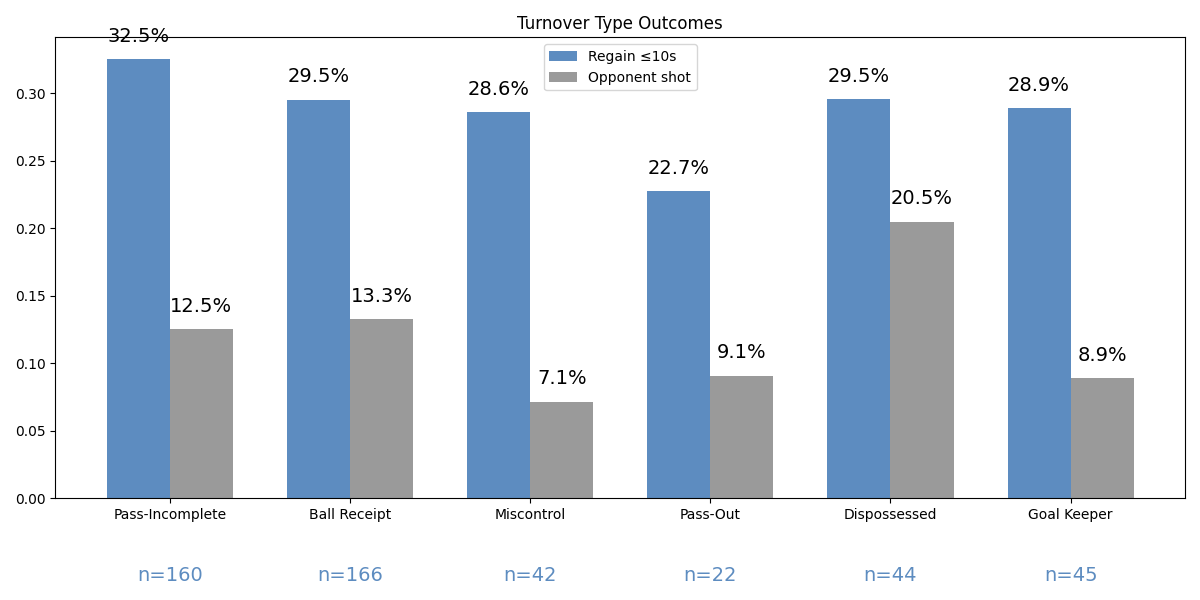
\includegraphics[width=50ex]{turnover_outcomes}\hfill
      Poor passing accounts for over 80\% of Villarreal's total possession losses, with a highly exploitable vulnerability corridor identified on the right flank. The team generally exhibits low ball-recovery rates within 10 seconds of a turnover, preferring to retreat into a structured defensive shape rather than aggressively counter-pressing. While this conservative approach successfully limits opponent shots for most turnover types, losing the ball via direct dispossession remains a critical tactical flaw. These one-on-one duel losses are exceptionally dangerous, resulting in poor recovery times and a disproportionately high rate of opponent shots.
     }
  \end{columns}

  % -- a wide block
  \block{Conclusion}
  	{
		While highly effective domestically, Villarreal’s possession-heavy tactical framework exposed severe structural vulnerabilities against elite Champions League opposition. Deep, patient build-up play frequently resulted in dangerous turnovers, particularly when players were forced into low-percentage long balls or trapped along the right flank. To bridge the gap to Europe's elite, the coaching staff must implement systematic counter-pressing triggers to accelerate post-loss recovery and stabilize defensive transitions.
	}
  \block{Ideas for Further Investigation}
	{
		Future research should leverage continuous tracking data to directly compare player recovery trajectories and fatigue levels in Champions League fixtures against their successful domestic matches. Additionally, evaluating the spatial positioning of opponent defensive blocks could isolate the exact pressing triggers that force Villarreal into high-volume passing errors.
	
	\begin{enumerate}
		\item introduction
	 	\item pitch control
		\item turnover types
		\item conclusion
	 	\item ideas for further investigation
	\end{enumerate}
	\begin{checkbox}
		sanity check
		spell check
	\end{checkbox}
	 }


% =================================================================
\end{document}
% =================================================================
